%\addcontentsline{toc}{chapter}{Development Process}
\chapter{Design and Experimental Methods}
\section{Design}
The ionic framework for developing mobile hybrid applications encourages the use of the Model View Controller (MVC) compound design pattern. MVC is something which is generally considered good practice within the software engineering industry and therefore the app was designed keeping that in mind.

The model of the app would be the database which is stored on the backend of the system. The view is the html files and the controllers are both the Angular JS controllers and the RESTful PHP API which I created.

\subsection{Overall Architecture}
Figure 2.1 shows the architecture as whole. Whilst figures X separates the model, view and controller.
\begin{figure}[H]
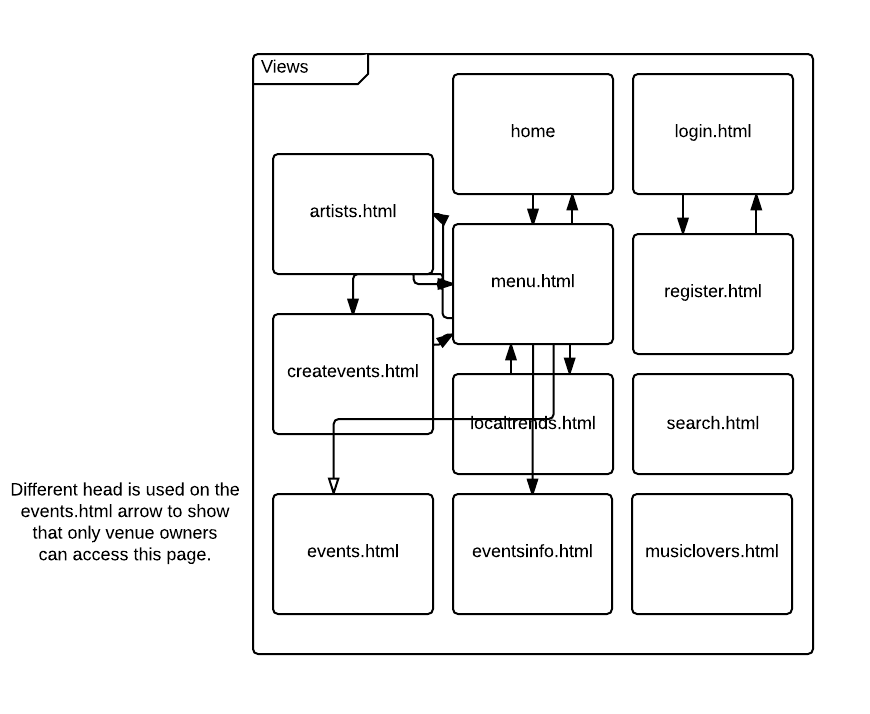
\includegraphics[width=\textwidth,height=\textheight,keepaspectratio]{images/va}
\caption{UML Diagram which illustrates the view. Created using https://www.lucidchart.com/}
\end{figure}
Figure 2.1 illustrates that once a user has logged in they can access multiple different pages through the menu bar (menu.html). The only page which is restricted is the events.html page as only venue owners can access this page to create events. The register.html page can only be accessed through the login page as it is accessed when a user needs to create a new account to login.

\subsection{Some detailed design}
The following figure highlights the different relationships between the tables (model) for events.
\begin{figure}[H]
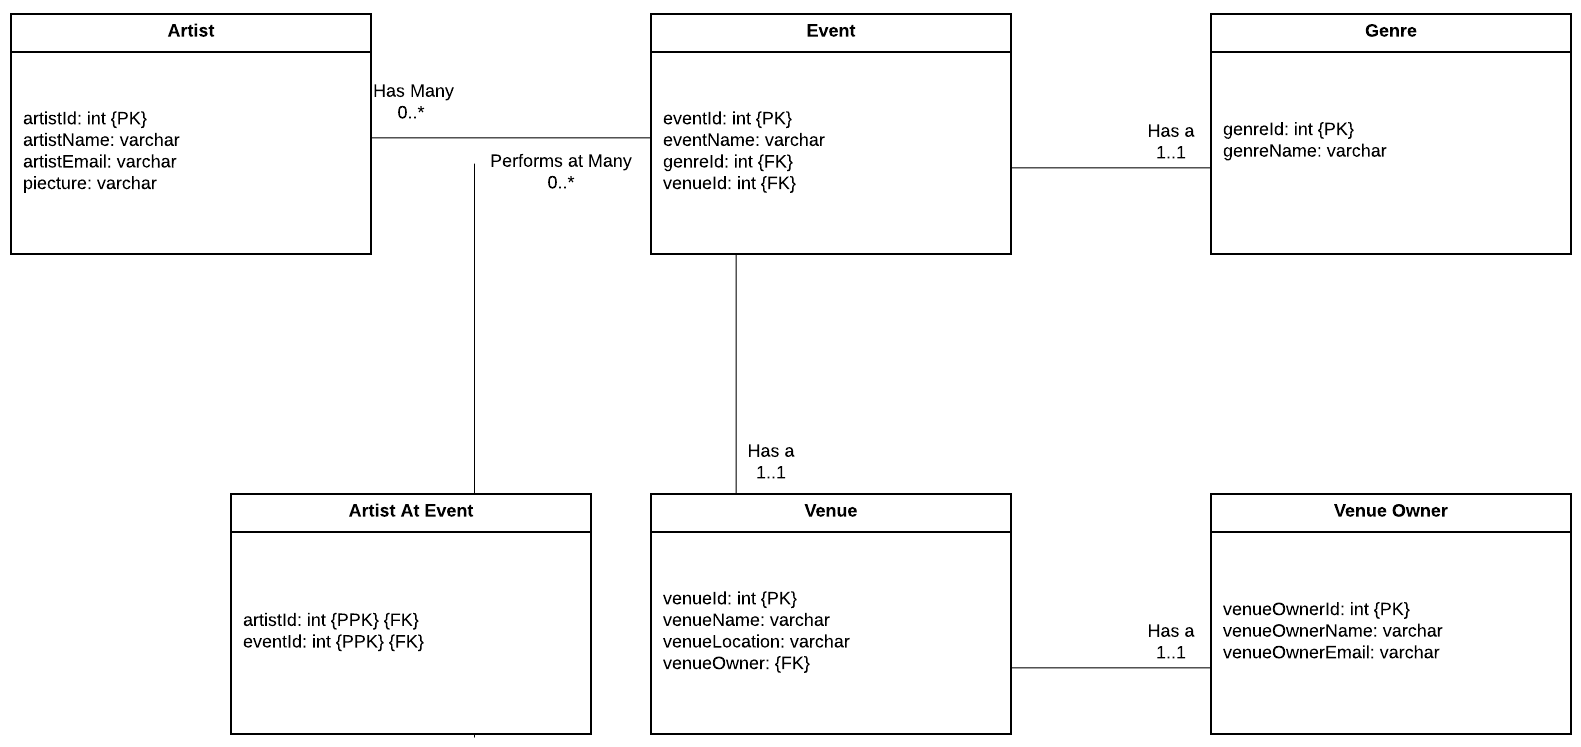
\includegraphics[width=\textwidth,height=\textheight,keepaspectratio]{images/events}
\caption{UML Diagram for the model in relation to events. Created using https://www.lucidchart.com/}
\end{figure}
Figure 2.2  is a UML diagram which shows the appropriate relationships between the different tables in the database in relation to an event.
\subsubsection{Even more detail}

\subsection{User Interface}
\begin{figure}[H]
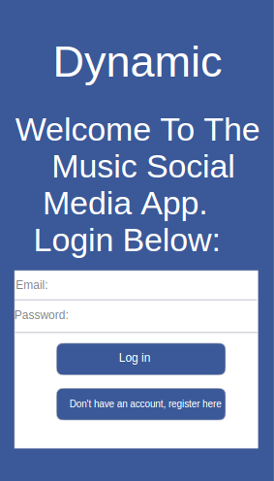
\includegraphics[scale=0.5]{images/ui1}
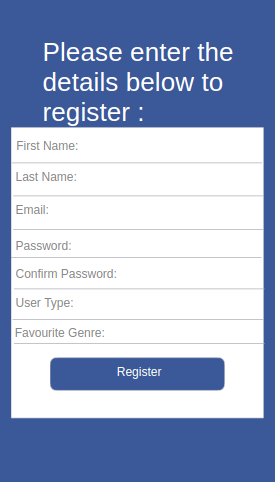
\includegraphics[scale=0.5]{images/ui2}
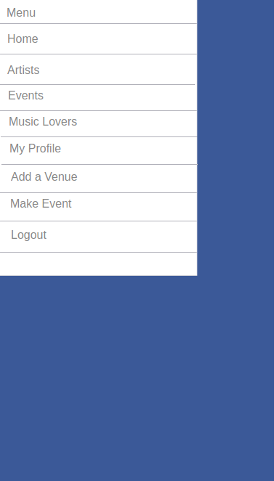
\includegraphics[scale=0.5]{images/ui3}
\caption{User interface mock up designed using https://www.fluidui.com}
\end{figure}

\section{Experimental Methods}
As the purpose of the project was to determine whether hybrid apps are feasible alternatives to native apps tests had to be derived. User testing is key to this as it allows for general users (people who use apps on a regular basis) to give feedback about whether they think the hybrid app is as good as a native app, if not why not etc. Another key aspect to answering the question is comparing the resource usage on the device of the hybrid app to a standard app, this will include comparing things such as amount of RAM being used.

Finally ,during each story in the development process, it was considered whether using hybrid app technology was as challenging, more challenging or less challenging than developing using native app technologies.
